\chapter{Lecture \thechapter{} of 07/04/2026}

\begin{proposition}[Book 1.4.13]
    
    Let $X,C \seq \Rn$ convex closed nonempty. Let $A \in \R^{m \times n}$, $m \in \N$, $m > 0$ and denote with $N(A)$ the nullspace of $A$. If $X$ is retractive and $\Rc{X} \cap \Rc{C} \cap N(A) \seq \Lc{C}$ then $A(X \cap C)$ is closed.

\end{proposition}

\begin{proof}
    
        Let $\set{y_k}_k \seq A(X \cap C)$ such that $y_k \to \bar{y}$ as $k \to +\infty$. To prove that $\bar{y} \in A(X \cap C)$, hence that there exists $\bar{x} \in X \cap C$ such that $A\bar{x} = \bar{y}$. Define $C_k = C \cap N_k$ where $N_k = \set{x : \norm{Ax - \bar{y}} \le \norm{y_k - \bar{y}}}$, these $C_K$ are convex and closed. Moreover $\Rc{C_k} = \Rc{C} \cap \Rc{N_k} = \Rc{C} \cap N(A)$. Use then point b) of proposition of the last lecture, and we are done. Why? $\norm{y_k - \bar{y}} \to 0$. For every $x \in C_k$, $\norm{Ax - \bar{y}} \le \norm{y_k - \bar{y}} \to 0$. For $x \in \bigcap_k C_k$, $\norm{Ax - \bar{y}}\le$ any value of a sequence that is going to 0, hence $\norm{Ax - \bar{y}} = 0 \implies Ax = \bar{y}$.

\end{proof}

\begin{remark}
    
    If $C = \Rn$, then $\Lc{C} = \Rn$, $X$ a polyhedral set (hence retractive), then $A(C \cap X) = A\times X$ is closed.

\end{remark}

\begin{remark}
    
    $X = \Rn$, $\Rc{X} = \Rn$. $A(X\ cap C) = AC$ closed if $\Rc \cap N(A) = \set{0}$.

\end{remark}

\begin{proposition}
    
    Let $C_1,\dots C_m$ be nonempty closed convex sets such that, if $d_1 + \dots + d_m = 0$ for $d_i \in \Rc{C_i}$ then $d_i \in \Lc{C_i}$, then $C_1 +\dots +C_m$ is closed.

\end{proposition}

\begin{proof}
    Not required.
\end{proof}

\begin{remark}
    
    If $C_1$ and $-C_2$ are closed and convex, then $C_1 - C_2$ is closed convex if $\Rc{C_1} \cap \Rc{C_2} = \set{0}$, so if one betweeen $C_1$ and $C_2$ is bounded.

\end{remark}

\begin{example}
    
    Let 

    \begin{align*}
        C_1 &= \set{(x,y) : x \ge 0,\, y \ge 1/x} \\
        C_2 &= \set{(x,y) : x = 0}.
    \end{align*}

    Then 

    \begin{align*}
        C_1 + C_2 &= \set{(x_1,y_1) + (x_2,y_2) : (x_1,y_1) \in C_1,\, (x_2,y_2) \in C_2} \\
            &= \set{(x_1,y_1 + \alpha) : (x_1,y_1) \in C_1,\, \alpha \in \R} \\
            &= \set{(x,y) : x > 0} 
    \end{align*}

    which is an open set. Observe that 

    \begin{align*}
        d_1 &= (0,1) \in \Rc{C_1} \\
        d_2 &= (0,-1) \in \Rc{C_2}.
    \end{align*}

    Then $d_1 + d_2 = 0$ and $d_2 \in \Lc{C_2}$ but $d_1 \notin \Lc{C_1}$.

\end{example}

\section{Hyperplanes}

An hyperplane is a set 

\[ H = \set{x : a^\top x = b} \]

for some $a \in \Rn$, $a \neq 0$, $b \in \R$. For $\bar{x} \in H$, we have 

\[ H = \set{x : a^\top x = a^\top \bar{x} } \]

hence $H = \bar{x} + \set{x : a^\top x = 0}$, where the latter is the parallel subspace to $H$. Furthermore we have the closed halfspaces where we replace the equal sign with a large inequality, closed with strict.

\subsection{Separation}

\begin{figure}[ht!]
    \centering
    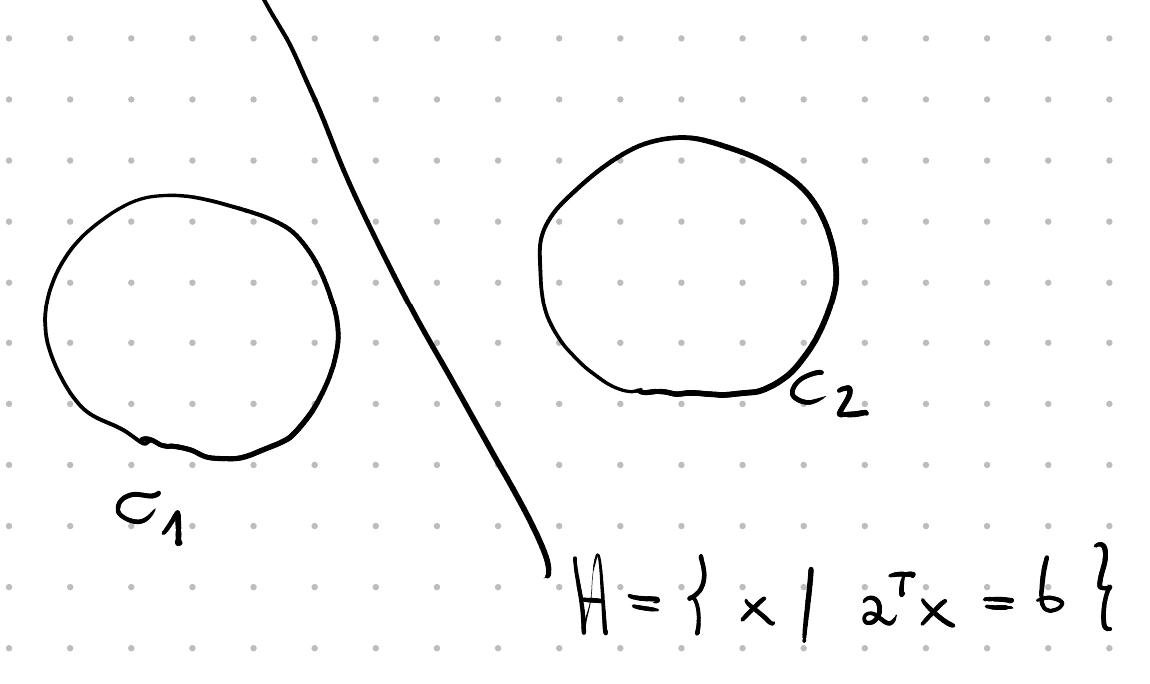
\includegraphics[width=0.6\textwidth]{img/separation.png}
    \caption{Hyperplane separating two closed convex sets}
\end{figure}

We say that $H$ separates $C_1$ and $C_2$ if $a^\top x_1 \le b \le a^\top x_2$ or the converse. We also write 

\[ \sup_{x_1 \in C_1} a^\top x_1 \le \inf_{x_2 \in C_2} a^\top x_2. \]

Assume $\bar{x} \in \cl{C}$ for $C \seq \Rn$. If $H$ separates $\set{\bar{x}}$ from $C$, we say $H$ is a supporting hyperplane at $\bar{x}$.

\begin{figure}[ht!]
    \centering
    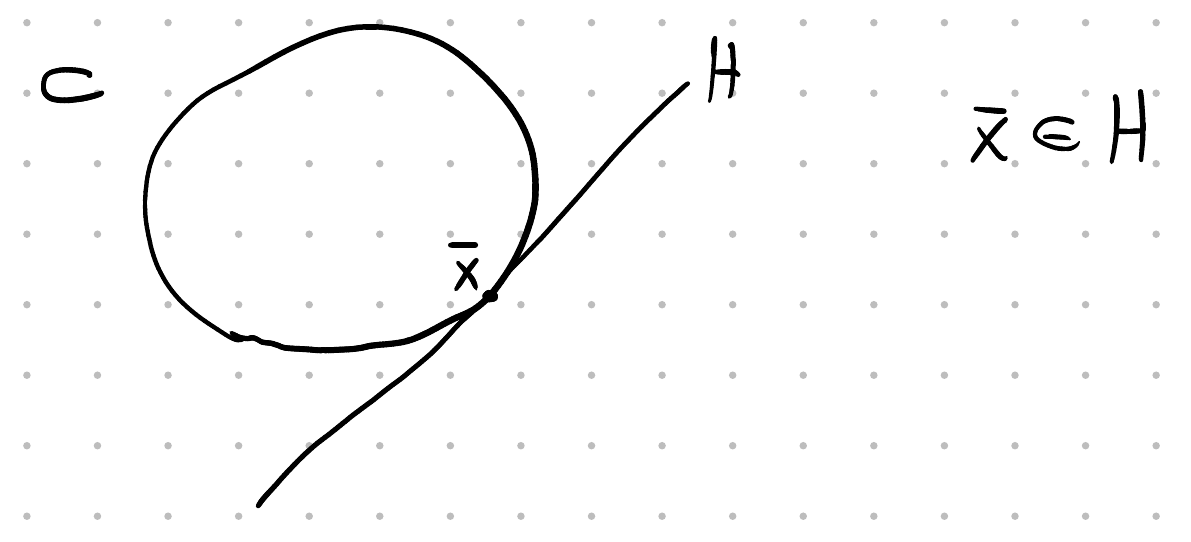
\includegraphics[width=0.6\textwidth]{img/supporting.png}
    \caption{Example of supporting hyperplane}
\end{figure}

\begin{proposition}[Supporting hyperplane theorem, book 1.5.1]
    
    Let $C \seq \Rn$ nonempty convex, $\bar{x} \in \Rn$, $x \notin \inter{C}$. Then there exists an hyperplane $H$ that passes through $\bar{x}$ and contains $C$ in one of its closed halfspaces, i.e. there exists $a \in \Rn$, $a \neq 0$ such that 

    \[ a^\top \bar{x} \le a^\top x \quad \forall x \in C. \]

\end{proposition}

\begin{proof}
    
    Consider $\bar{x} \notin \inter{C}$. One can prove that there exists a sequence $\set{x_k}_k \seq \Rn \smallsetminus \cl{C}$ such that $x_k \to \bar{x}$. (to prove this, later...)

    Consider $\hat{x}_k$ the projection of $x_k$ onto $\cl{C}$ which is a closed convex set, so the projection exists and it is uniqe. By projection theorem, it holds that 

    \[ \langle \hat{x}_k - x_k, x - \hat{x}_k \rangle \ge 0 \quad \forall x \in \cl{C}. \]

    Rewrite

    \begin{align*}
        (\hat{x}_k - x_k)^\top \cdot x &\ge (\hat{x}_k - x_k)^\top \cdot (\hat{x}_k \pm x_k) \\
            &= \underbrace{(\hat{x}_k - x_k)^\top\cdot(\hat{x}_k - x_k)}_{\ge 0} + (\hat{x}_k - x_k)^\top\cdot x_k \\
            &\ge (\hat{x}_k - x_k)^\top\cdot x_k
    \end{align*}

    Define $a_k = \displaystyle\frac{\hat{x}_k - x_k}{\norm{\hat{x}_k - x_k}}$, we obtain that $a_k^\top \cdot x \ge a_k^\top \cdot x_k$ for any $x \in \cl{C}$ and for any $k$. The sequence $\set{a_k}_k \seq \overline{B(0,1)}$, so by BW, up to subsequences, $a_k \to \bar{a} \in \Rn$, $\norm{\bar{a}} = 1$. Taking the limit 

    \[ 
        \begin{array}{ccc}
            a^\top_k \cdot x & \ge & \a^\top_k x_k \\
            \downarrow & & \downarrow \\
            \bar{a}^\top\cdot x & \ge &\bar{a}^\top \cdot \bar{x}.
        \end{array}
    \]

    Hence $\bar{a}$ defines our target hyperplane.

\end{proof}

\begin{proposition}[Separating hyperplane theorem (finite HB), Book 1.5.2]

    Let $C_1,C_2 \seq \Rn$ be nonempty convex. If $C_1$ and $C_2$ are disjoint, then there exists $a \in \Rn$, $a \neq 0$ such that 

    \[ a^\top x_1 \le a^\top x_2 \quad \forall x_1 \in C_1 \, \forall x_2 \in C_2. \]
    
\end{proposition}

\begin{proof}
    
    Let $C = C_1 - C_2$ the algebraic set difference. Observe that $0 \notin C$, as $C_1 \cap C_2 = \emptyset$. Let $H$ be the hyperplane separating $\set{0}$ and $C$, so there exists $a \in \Rn \setminus\set{0}$ such that $0 \le a^\top x$ for all $x \in C$. Every $x \in C$ is in the form $x = x_1 - x_2$, hence 

    \[ 0 \le a^\top (x_1 - x_2) \iff a^\top x_2 \le a^\top x_1. \]

\end{proof}

\begin{example}
    
    Let 

    \begin{align*}
        C_1 &= \set{(x,y) : y \ge e^x} \\
        C_2 &= \set{(x,y) : y \le 0}.
    \end{align*}

    Then $C_1 \cap C_2 = \emptyset$ and $H = \set{(x,y) : y = 0}$.

\end{example}

\begin{proposition}[Strict separation theorem, book 1.5.3]
    
    Let $C_1,C_2 \seq \Rn$ convex disjoint. Then $C_1$ and $C_2$ can be strictly separated if one of the following holds:
    
    \begin{enumerate}
        \item $C_1 - C_2$ is closed;
        \item $C_1$ closed and $C_2$ compact;
        \item $C_1,C_2$ polyhedral;
        \item $C_1,C_2$ closed and $\Rc{C_1} \cap \Rc{C_2} = \Lc{C_1} \cap \Lc{C_2}$;
        \item $C_1$ is closed, $C_2$ polyhedral, $\Rc{C_1} \cap \Rc{C_2} \seq \Lc{C_1}$.
    \end{enumerate}

\end{proposition}

\begin{proof}
    
    We only prove under condition $2)$: assume $C_1 = A$ closed and $C_2 = B$ compact. Define 

    \[ d^* = \inf_{a \in A,\, b \in B} \norm{a-b} \ge 0. \]

    Consider a maximizing sequence $(a_k,b_k)$ where $a_k \in A$, $b_k \in B$ such that $\norm{a_k - b_k} \to d^*$. Since $B$ is compact, $\set{b_k}_k$ is bounded, hence, up to subsequences, $b_k \to \bar{b} \in B$, since $B$ is closed. This implies also that $\set{a_k}_k$ is bounded (otherwise $\norm{a_k - b_k} \to +\infty$), so, up to subsequences, $a_k \to \bar{a} \in A$. We have shown that $\norm{a_k - b_k} \to \norm{\bar{a} - \bar{b}}$. But, observing that $\norm{a_k - b_k} \to d^*$, by uniqueness of the limit, we have also that $d^* = \norm{\bar{a} - \bar{b}}$. In particular $\bar{a}$ is the projection of $\bar{b}$ onto $A$, and $\bar{b}$ is the projection of $\bar{a}$ onto $B$. By projection theorem, 

    \begin{align*}
        (\bar{b} - \bar{a})^\top \cdot (a - \bar{a}) &\le 0 \quad \forall a \in A \\
        (\bar{a} - \bar{b})^\top \cdot (b - \bar{b}) &\le 0 \quad \forall b \in B.
    \end{align*}

    Consider $c = \bar{b} - \bar{a}$. Pick $\bar{x}$ on the segment connection $\bar{a}$ to $\bar{b}$, then 

    \[ H = \bar{x} + \set{x : c^\top x = 0} \]

    strictly separates $A$ and $B$.

\end{proof}

\begin{proposition}[Book 1.5.4]

    The closure of the conves hull of a set $C$ is the intersection of all the closed halfspaces containing $C$.

\end{proposition}

\begin{proof}
    
    \begin{align*}
        H &= \text{ intersection of closed halspaces containing } C \\
            &= \bigcap \set{\tilde{H} \text { s.t. } \tilde{H} \text{ is a closed halfspace, } C \seq H}.
    \end{align*}

    We prove the double inclusion. 

    \paragraph{$\cl{\conv{C}} \seq H$:} if $\tilde{H}$ is a closed subspace containing $C$, then $\tilde{H}$ contains $\cl{\conv{C}}$, so $\cl{\conv{C}}$ is contained also in their intersection, which is $H$.

    \paragraph{$H \seq \cl{\conv{C}}$:} we prove that $\Rn \setminus \cl{\conv{C}} \seq \Rn \setminus H$. Let $x \in \Rn \setminus \cl{\conv{C}}$. Since $x \notin \cl{\conv{C}}$, by strict separation point 2., we can separate $\set{x}$ from $\cl{\conv{C}}$ via an hyperplane $H^*$, which is contained in $H$. The halfspace corresponding to $H^*$ does not contain $x$, so $x \notin H$. Hence $H \seq \cl{\conv{C}}$.

\end{proof}
